\documentclass{article}

\usepackage[a4paper,left=1in,right=1in,top=1in,bottom=1in]{geometry}

\usepackage{amsmath}
\usepackage{amsfonts}
\usepackage{amssymb}
\usepackage{xcolor}
\usepackage{graphicx}

\usepackage{amsmath,amsfonts,amssymb,amsthm}
\usepackage{fullpage}
\usepackage{times}
\usepackage{hyperref}
\usepackage{pdfsync}
\usepackage{microtype}
\usepackage{color}
\usepackage{cleveref}
\crefformat{footnote}{#2\footnotemark[#1]#3}
\definecolor{light-gray}{gray}{0.5}

%%% BLACKBOARD SYMBOLS

\newcommand{\C}{\ensuremath{\mathbb{C}}}
\newcommand{\D}{\ensuremath{\mathbb{D}}}
\newcommand{\F}{\ensuremath{\mathbb{F}}}
\newcommand{\G}{\ensuremath{\mathbb{G}}}
\newcommand{\J}{\ensuremath{\mathbb{J}}}
\newcommand{\N}{\ensuremath{\mathbb{N}}}
\newcommand{\Q}{\ensuremath{\mathbb{Q}}}
\newcommand{\R}{\ensuremath{\mathbb{R}}}
\newcommand{\T}{\ensuremath{\mathbb{T}}}
\newcommand{\Z}{\ensuremath{\mathbb{Z}}}
\newcommand{\QR}{\ensuremath{\mathbb{QR}}}

\newcommand{\Zt}{\ensuremath{\Z_t}}
\newcommand{\Zp}{\ensuremath{\Z_p}}
\newcommand{\Zq}{\ensuremath{\Z_q}}
\newcommand{\ZN}{\ensuremath{\Z_N}}
\newcommand{\Zps}{\ensuremath{\Z_p^*}}
\newcommand{\ZNs}{\ensuremath{\Z_N^*}}
\newcommand{\JN}{\ensuremath{\J_N}}
\newcommand{\QRN}{\ensuremath{\QR_{N}}}
\newcommand{\QRp}{\ensuremath{\QR_{p}}}

%%% THEOREM COMMANDS

\theoremstyle{plain}            % following are "theorem" style
\newtheorem{theorem}{Theorem}[section]
\newtheorem{lemma}[theorem]{Lemma}
\newtheorem{corollary}[theorem]{Corollary}
\newtheorem{proposition}[theorem]{Proposition}
\newtheorem{claim}[theorem]{Claim}
\newtheorem{fact}[theorem]{Fact}

\theoremstyle{definition}       % following are def style
\newtheorem{definition}[theorem]{Definition}
\newtheorem{conjecture}[theorem]{Conjecture}
\newtheorem{example}[theorem]{Example}
\newtheorem{protocol}[theorem]{Protocol}

\theoremstyle{remark}           % following are remark style
\newtheorem{remark}[theorem]{Remark}
\newtheorem{note}[theorem]{Note}
\newtheorem{exercise}[theorem]{Exercise}

% equation numbering style
\numberwithin{equation}{section}

%%% GENERAL COMPUTING

\newcommand{\bit}{\ensuremath{\set{0,1}}}
\newcommand{\pmone}{\ensuremath{\set{-1,1}}}

% asymptotics
\DeclareMathOperator{\poly}{poly}
\DeclareMathOperator{\polylog}{polylog}
\DeclareMathOperator{\negl}{negl}
\newcommand{\Otil}{\ensuremath{\tilde{O}}}

% probability/distribution stuff
\DeclareMathOperator*{\E}{E}
\DeclareMathOperator*{\Var}{Var}

% sets in calligraphic type
\newcommand{\calD}{\ensuremath{\mathcal{D}}}
\newcommand{\calF}{\ensuremath{\mathcal{F}}}
\newcommand{\calH}{\ensuremath{\mathcal{H}}}
\newcommand{\calK}{\ensuremath{\mathcal{K}}}
\newcommand{\calM}{\ensuremath{\mathcal{M}}}
\newcommand{\calX}{\ensuremath{\mathcal{X}}}
\newcommand{\calY}{\ensuremath{\mathcal{Y}}}

% types of indistinguishability
\newcommand{\compind}{\ensuremath{\stackrel{c}{\approx}}}
\newcommand{\statind}{\ensuremath{\stackrel{s}{\approx}}}
\newcommand{\perfind}{\ensuremath{\equiv}}

% font for general-purpose algorithms
\newcommand{\algo}[1]{\ensuremath{\mathsf{#1}}}
% font for general-purpose computational problems
\newcommand{\problem}[1]{\ensuremath{\mathsf{#1}}}
% font for complexity classes
\newcommand{\class}[1]{\ensuremath{\mathsf{#1}}}

% complexity classes and languages
\renewcommand{\P}{\class{P}}
\newcommand{\BPP}{\class{BPP}}
\newcommand{\NP}{\class{NP}}
\newcommand{\coNP}{\class{coNP}}
\newcommand{\AM}{\class{AM}}
\newcommand{\coAM}{\class{coAM}}
\newcommand{\IP}{\class{IP}}

%%% "LEFT-RIGHT" PAIRS OF SYMBOLS

% inner product
\newcommand{\inner}[1]{\langle{#1}\rangle}
\newcommand{\innerfit}[1]{\left\langle{#1}\right\rangle}
% absolute value
\newcommand{\abs}[1]{\lvert{#1}\rvert}
\newcommand{\absfit}[1]{\left\lvert{#1}\right\rvert}
% a set
\newcommand{\set}[1]{\{{#1}\}}
\newcommand{\setfit}[1]{\left\{{#1}\right\}}
% parens
\newcommand{\parens}[1]{({#1})}
\newcommand{\parensfit}[1]{\left({#1}\right)}
% tuple = alias for parens
\newcommand{\tuple}[1]{\parens{#1}}
\newcommand{\tuplefit}[1]{\parensfit{#1}}
% square brackets
\newcommand{\bracks}[1]{[{#1}]}
\newcommand{\bracksfit}[1]{\left[{#1}\right]}
% rounding off
\newcommand{\round}[1]{\lfloor{#1}\rceil}
% floor function
\newcommand{\floor}[1]{\lfloor{#1}\rfloor}
% ceiling function
\newcommand{\ceil}[1]{\lceil{#1}\rceil}
% length of a string
\newcommand{\len}[1]{\lvert{#1}\rvert}
\newcommand{\lenfit}[1]{\left\lvert{#1}\right\rvert}
% length of some vector, element
\newcommand{\length}[1]{\lVert{#1}\rVert}
\newcommand{\lengthfit}[1]{\left\lVert{#1}\right\rVert}

%%% CRYPTO-RELATED NOTATION

% KEYS AND RELATED

\newcommand{\key}[1]{\ensuremath{#1}}

\newcommand{\pk}{\key{pk}}
\newcommand{\vk}{\key{vk}}
\newcommand{\sk}{\key{sk}}
\newcommand{\mpk}{\key{mpk}}
\newcommand{\msk}{\key{msk}}
\newcommand{\fk}{\key{fk}}
\newcommand{\id}{id}
\newcommand{\keyspace}{\ensuremath{\mathcal{K}}}
\newcommand{\msgspace}{\ensuremath{\mathcal{M}}}
\newcommand{\ctspace}{\ensuremath{\mathcal{C}}}
\newcommand{\tagspace}{\ensuremath{\mathcal{T}}}
\newcommand{\idspace}{\ensuremath{\mathcal{ID}}}

\newcommand{\concat}{\ensuremath{\|}}

% GAMES

% advantage
\newcommand{\advan}{\ensuremath{\mathbf{Adv}}}

% different attack models
\newcommand{\attack}[1]{\ensuremath{\text{#1}}}

\newcommand{\atk}{\attack{atk}} % dummy attack
\newcommand{\indcpa}{\attack{ind-cpa}}
\newcommand{\indcca}{\attack{ind-cca}}
\newcommand{\anocpa}{\attack{ano-cpa}} % anonymous
\newcommand{\anocca}{\attack{ano-cca}}
\newcommand{\euacma}{\attack{eu-acma}} % forgery: adaptive chosen-message
\newcommand{\euscma}{\attack{eu-scma}} % forgery: static chosen-message
\newcommand{\suacma}{\attack{su-acma}} % strongly unforgeable

% ADVERSARIES
\newcommand{\attacker}[1]{\ensuremath{\mathcal{#1}}}

\newcommand{\Adv}{\attacker{A}}
\newcommand{\AdvA}{\attacker{A}}
\newcommand{\AdvB}{\attacker{B}}
\newcommand{\Dist}{\attacker{D}}
\newcommand{\Sim}{\attacker{S}}
\newcommand{\Ora}{\attacker{O}}
\newcommand{\Inv}{\attacker{I}}
\newcommand{\For}{\attacker{F}}

% CRYPTO SCHEMES

\newcommand{\scheme}[1]{\ensuremath{\text{#1}}}

% pseudorandom stuff
\newcommand{\prg}{\algo{PRG}}
\newcommand{\prf}{\algo{PRF}}
\newcommand{\prp}{\algo{PRP}}

% symmetric-key cryptosystem
\newcommand{\skc}{\scheme{SKC}}
\newcommand{\skcgen}{\algo{Gen}}
\newcommand{\skcenc}{\algo{Enc}}
\newcommand{\skcdec}{\algo{Dec}}

% public-key cryptosystem
\newcommand{\pkc}{\scheme{PKC}}
\newcommand{\pkcgen}{\algo{Gen}}
\newcommand{\pkcenc}{\algo{Enc}} % can also use \kemenc and \kemdec
\newcommand{\pkcdec}{\algo{Dec}}

% digital signatures
\newcommand{\sig}{\scheme{SIG}}
\newcommand{\siggen}{\algo{Gen}}
\newcommand{\sigsign}{\algo{Sign}}
\newcommand{\sigver}{\algo{Ver}}

% message authentication code
\newcommand{\mac}{\scheme{MAC}}
\newcommand{\macgen}{\algo{Gen}}
\newcommand{\mactag}{\algo{Tag}}
\newcommand{\macver}{\algo{Ver}}

% key-encapsulation mechanism
\newcommand{\kem}{\scheme{KEM}}
\newcommand{\kemgen}{\algo{Gen}}
\newcommand{\kemenc}{\algo{Encaps}}
\newcommand{\kemdec}{\algo{Decaps}}

% identity-based encryption
\newcommand{\ibe}{\scheme{IBE}}
\newcommand{\ibesetup}{\algo{Setup}}
\newcommand{\ibeext}{\algo{Ext}}
\newcommand{\ibeenc}{\algo{Enc}}
\newcommand{\ibedec}{\algo{Dec}}

% hierarchical IBE (as key encapsulation)
\newcommand{\hibe}{\scheme{HIBE}}
\newcommand{\hibesetup}{\algo{Setup}}
\newcommand{\hibeext}{\algo{Extract}}
\newcommand{\hibeenc}{\algo{Encaps}}
\newcommand{\hibedec}{\algo{Decaps}}

% binary tree encryption (as key encapsulation)
\newcommand{\bte}{\scheme{BTE}}
\newcommand{\btesetup}{\algo{Setup}}
\newcommand{\bteext}{\algo{Extract}}
\newcommand{\bteenc}{\algo{Encaps}}
\newcommand{\btedec}{\algo{Decaps}}

% trapdoor functions
\newcommand{\tdf}{\scheme{TDF}}
\newcommand{\tdfgen}{\algo{Gen}}
\newcommand{\tdfeval}{\algo{Eval}}
\newcommand{\tdfinv}{\algo{Invert}}
\newcommand{\tdfver}{\algo{Ver}}

%%% PROTOCOLS

\newcommand{\out}{\text{out}}
\newcommand{\view}{\text{view}}


\title{Identification and Signature based On MQ Problem}
\author{Manish Kumar (21044)}

\begin{document}

\maketitle

\section*{Abstract} Multivariate Quadratic Identification protocol (MQ-IDS) and Digital Signature (MQ-DSS) scheme are part of Multivariate public key cryptography (MPKC). MPKC is considered a prospective candidate for post quantum cryptography.\footnote{Bernstein, Buchmann and Dahmen, Post Quantum Cryptography (Springer), Chapter-8} Even MQ-DSS was a second round candidate in NIST post quantum cryptography standarisation project.
\footnote{https://csrc.nist.gov/CSRC/media/Presentations/mqdss-round-2-presentation/images-media/mqdss-hulsing.pdf} A secure public key crpytosystem requires a secure trapdoor function. In this scribe, we will discuss a trapdoor based on Multivariate quadratics. We will do security analysis of a 3-pass IDS (Sakumoto et.al) in terms of Zero Knowledge and Proof of Knowledge. This IDS can be extended to create MQ-DSS. Finally we do brief analysis of 5-pass IDS in signature construction which was floated as an exercise. 
\section*{Knowing The Trapdoor Function: The Multivariate Quadratic Problem}
Consider the below m-systems of Multivariate polynomial in n-variables over a finite field $\mathbb{F}_q$ :
\[ f^{1}(x_1,...,x_n) = \sum_{i=1}^{n} \sum_{i=1}^{n} \alpha^{(1)}_{ij} x_i x_j + \sum_{i=1}^{n} \beta^{(1)}_i x_i +\gamma^{(1)} \]
\[ ... \]
\[ f^{m}(x_1,...,x_n) = \sum_{i=1}^{n} \sum_{i=1}^{n} \alpha^{(m)}_{ij} x_i x_j + \sum_{i=1}^{n} \beta^{(m)}_i x_i +\gamma^{(m)} \]
$MQ\ problem$ is a task to compute $\hat{x} = (x_1,...,x_n)$ from $y = (y_1,..y_m)$ such that $ f^{k}(\hat{x})=y_k, \forall\ k \in \{1,...,m\} $, where all coefficients and variables belongs to finite field $\mathbb{F}_q$. The problem is originally from computational algebraic geometry. It has been shown that the decision version of $MQ\ problem$ is NP-hard. Based on current known state of art classical and quantum algorithms, it is conjectured that $MQ\ problem$ has no efficient solution. The problem would get much harder if we increase the order of polynomial to cubic, quartic or above. But public key $(pk)$ size would also increase accordingly. Since any polynomial is defined uniquely by its coefficients. Hence, the set of coefficients and $\mathbb{F}_q$ is part of $pk$. In case of a d-degree polynomial with n-variables, number of all the coefficients is ${n+d \choose d}$. Hence, for m-sets of d-degree polynomials, size of $pk$ roughly varies $\sim O(mn^d)$. The best balance between desired toughness of the problem and manageable key size is achieved for $d=2$, i.e, Quadratic. The case of $d=1$ is called system of linear equations. It has an efficient classical as well as quantum solution. \footnote{https://arxiv.org/abs/0811.3171}
\section*{3-pass IDS of Sakumoto, Shirai and Hiwatari (2011) \footnote{https://www.iacr.org/archive/crypto2011/68410703/68410703.pdf}}
It is a challenge-response based interactive identification protocol. We will discuss its three components namely Key-Gen, Identification and Verification.\\
\textbf{Key-Gen:} It takes a security parameter $\kappa$ (say) and generate $\textbf{F} \in_R \textbf{MQ}(m,n,\mathbb{F}_q)$, which is m-tuple of random multivariate quadratic polynomials. Then a random vector $s \in_R \mathbb{F}^n _q$ is used to generate $v$ such that  $v = \textbf{F}(s)$. Finally the output of Key-Gen as $(pk,\ sk) = (v,\ s)$.\\
\textbf{Identification:} The prover $\mathcal{P}$ has to prove she has secret $s$ without revealing it to verifier $\mathcal{V}$. Since interactive proofs employs cut-and-choose protocol where a prover first divides her secret into shares and then proves the correctness of some shares depending on the choice of a verifier without revealing the secret itself. The dividing technique employed here is based on bilinearity of polar form of MQ function. The polar form $\textbf{G}$ and MQ function $\textbf{F}$ satisfy the relation $ \textbf{G}(x_1,x_2) = \textbf{F}(x_1 + x_2) -\textbf{F}(x_1)-\textbf{F}(x_2)$.\\
$\bullet$ The interaction starts when $\mathcal{P}$ makes a commitment $ct$. For $ct$, she pick $\textbf{a}_0, \textbf{b}_0 \in_R \mathbb{F}^n _q$ and $\textbf{c}_0 \in_R \mathbb{F}^m _q$. Now she embed secret $s$ as $\textbf{a}_1 =\textbf{s}-\textbf{a}_0$ and $\textbf{b}_1 = \textbf{a}_0 - \textbf{b}_0$. These parameters are used to create $\textbf{c}_1 = \textbf{F}(\textbf{a}_0)-\textbf{c}_0$, $\textbf{ct}_0 = H(\textbf{a}_1 \parallel \textbf{G}(\textbf{b}_0, \textbf{a}_1) + \textbf{c}_0)$, $\textbf{ct}_1 = H(\textbf{b}_0\parallel \textbf{c}_0)$ and $\textbf{ct}_2 = H(\textbf{b}_1\parallel \textbf{c}_1)$. Finally, $\textbf{ct} = (ct_0, ct_1, ct_2)$ is send to $\mathcal{V}$ as commitment. Here, $H$ is a collision resistant hash function (CRHF). In principle, we can use any function instead of $H$. But that function should have $statistically\ hiding$ as well as $computationally\ binding$ property.\\
$\bullet$ After $\mathcal{V}$ receives $\textbf{ct}$, he sends a random challenge $\textbf{ch} \in_R \{0,1,2\}$.\\
$\bullet$ Based on received $\textbf{ch}$, $\mathcal{P}$ sends response $rs$. If $ch =0$, $rs=(\textbf{a}_0,\textbf{b}_1,\textbf{c}_1)$.
If $ch =1$, $rs=(\textbf{a}_1,\textbf{b}_1,\textbf{c}_1)$. If $ch =2$, $rs=(\textbf{a}_1,\textbf{b}_0,\textbf{c}_0)$.\\
\textbf{Verification:} Now, $\mathcal{V}$ checks the response $rs$ as per below criteria, and then accordingly declare if verification is successful or not. Failure at any single stage is taken as failure of the verification process.\\
$\bullet$ If $ch$ =0, parse $rs$ as $(\textbf{a}_0,\textbf{b}_1,\textbf{c}_1)$ and check, if $ct_1 \stackrel{?}{=} H(\textbf{a}_0 - \textbf{b}_1 \parallel \textbf{F}(\textbf{a}_0) -\textbf{c}_0)$, and $ct_2 = H(\textbf{b}_1 \parallel \textbf{c}_1)$.\\
$\bullet$ If $ch$ =1, parse $rs$ as $(\textbf{a}_1,\textbf{b}_1,\textbf{c}_1)$ and check, if $ct_0 \stackrel{?}{=} H(\textbf{a}_1 \parallel \textbf{v}- \textbf{F}(\textbf{a}_1) - \textbf{G}(\textbf{b}_1, \textbf{a}_1) -\textbf{c}_0)$, and $ct_2 = H(\textbf{b}_1 \parallel \textbf{c}_1)$.\\
$\bullet$ If $ch$ =2, parse $rs$ as $(\textbf{a}_1,\textbf{b}_0,\textbf{c}_0)$ and check, if $ct_0 \stackrel{?}{=} H(\textbf{a}\parallel \textbf{G}(\textbf{b}_0), \textbf{a}_1) + \textbf{c}_0$, and $ct_1 = H(\textbf{b}_0 \parallel \textbf{c}_0)$.\\
\\
\textbf{Security analysis:} We expect $zero\ knowledge$ and $proof\ of\ knowledge$ from a secure Identification scheme. MQ-IDS meets both of the requirement as analysed below.\\

$\star\ $ $\underline{Honest\ verifier\ zero\ knowledge}$ (HVZK): The proof strategy is based on the logic that if two data-set have similar distribution, then the statistical insight we get from one data-set can be inferred from the other data-set as well. Hence, owing one of the data-set provides no more advantage over the other data-set. To be more precise, Let the data harvested by an adversary $\mathcal{A}$ by participating in the identification process be\\
$\mathcal{A} := \{(pk, sk, \pi): (pk,sk)\leftarrow Key-Gen; \pi\leftarrow Trans(\left\langle P(pk,sk),V(pk)\right\rangle)\}$\\
And, a simulator generated, $\mathcal{S} := \{(pk, sk, \pi): (pk,sk)\leftarrow Key-Gen; \pi\leftarrow Simulate(pk)\}$\\
If $\mathcal{A}$ and $\mathcal{S}$ are indistinguishable distribution, then we can say no statistically significant knowledge can be gained by participating in the protocol. Now we will see such $\mathcal{S}$ is possible to construct as follow:\\
If we look closely at the challenge-response protocol, we can make three interesting statistical observation. First, the challenge $\textbf{a}_0, \textbf{b}_0, \textbf{c}_0, \textbf{a}_1 $ and $ \textbf{b}_1$ are random. Only $\textbf{a}_1$ is influenced by secret key $\textbf{s}$. Second, challenge $ch$ is picked and send randomly from $\{0,1,2\}$, and the three possible response $rs$ collectively have uniform distribution of its components $\textbf{a}_i, \textbf{b}_i$ and $ \textbf{c}_i$. Third, the $H$ function acts like a random function with hiding property. The simulator generates a proof as:\\
$\bullet$ It chooses a $ch \in_R \{0,1,2\}$ and a fake secret $\textbf{s'} \in \mathbb{F}^n _q$.\\
$\bullet$ if $ch \in \{0,2\}$ then $ct = (ct_0, ct_1, ct_2)$ and response $rs$ are generated exactly like the protocol employing $\textbf{s'}$.\\
$\bullet$ If $ch =1$, then $rs$ and $ct_2$ are generated as in protocol but $ct_0$ is computed as done during verification as $ct_0= H(\textbf{a}_1 \parallel \textbf{v}- \textbf{F}(\textbf{a}_1) - \textbf{G}(\textbf{b}_1, \textbf{a}_1) -\textbf{c}_0)$.\\
Here, $H$ acting as a random function is making sure that $ct$ doesn't convey any information of $\textbf{s'}$ and corresponding response $rs$. It implies there is no efficient way to distinguish the original proof and the one simulated by the above method. Hence, $zero\ knowledge$ is guaranteed.\\

$\star\ $ $\underline{Proof\ of\ knowledge}$ (via 3-special Soundness): The idea stems from soundness of a proof system in Logic. For an IDS = (Key-Gen, P, V), it is said to be sound with knowledge error $k$ if all probabilistic polynomial time (PPT) adversary $\mathcal{A}$ we have: $P[b=1:(pk, sk)\leftarrow Key-Gen;b\leftarrow \left\langle \mathcal{A}(pk,\perp);V(pk) \right\rangle]\leq k+ \epsilon$ ; $\epsilon \rightarrow 0$. In other words, if a person possess the secret key then the verifier always output success ($b=1$), otherwise the maximum probability of success without knowing $s$ is upper bounded by $k + \epsilon$.\\
$\bullet$ 3-pass MQ-IDS satisfies 3-special soundness property. It means if we somehow harvest three $special$ valid transcript then we can build an extractor that can efficiently compute witness $sk$. Three special transcripts are: $\pi = (ct,ch,rs)$, $\pi^{'} = (ct,ch',rs')$ and $\pi^{"} = (ct,ch",rs")$ with $ch\neq ch'\neq ch"$.\\ 
$\bullet$ The recovery of witness $sk$ from valid transcripts: Start with transcripts $(ct,0,rs_0);\ (ct,1,rs_1);$ and $(ct,2,rs_2)$. Where $ct= (ct_0,ct_1, ct_2)$, $rs_0= (a^{(0)} _0, b^{(0)} _1, c^{(0)} _1 )$, $(a^{(1)} _1, b^{(1)} _1, c^{(1)} _1 )$, and $(a^{(2)} _1, b^{(2)} _0, c^{(0)} _0)$.
Being a valid transcript it must satisfy the corresponding verification equations. We compare the case of $ch=1$ and $ch=2$, we see $ct_0$ is part of both of them. Hence, they must be equal. Comparing them yields,\\
$ct_0 = H(\textbf{a}^{(1)}_1 \parallel \textbf{v}- \textbf{F}(\textbf{a}^{(1)} _1) - \textbf{G}(\textbf{b}^{(1)} _1, \textbf{a}^{(1)} _1) -\textbf{c}^{(1)} _1)$ = $ H(\textbf{a}^{(2) _1} \parallel \textbf{G}(\textbf{b}^{(1)} _0), \textbf{a}^{(1)} _1) + \textbf{c}^{(1)} _0$. \\ 
It implies $a^{(1)}_1 = a^{(2)}_1$ and $v= F(a^{(1)} _1) + G(b^{(1)} _1, a^{(1)} _1) + c^{(1)} _1 + G(b^{(1)} _0, a^{(1)} _1 ) + c^{(2)} _0$\\
If we do the above analysis for other two cases of $(ch=0, ch=2)$ and $(ch=0, ch=1)$, we get more relationship between the parameters. After suitable substitution and elimination within the set of relations, we get $v=F(a^{(0)} _0 + a^{(1)} _1)$. 
 The result simply says $a^{(0)} _0 + a^{(1)} _1$ is a preimage of $v$. Hence, it is a witness.[QED]\\
 $\bullet$ Argument for proof of knowledge: We assume MQ problem is intractable. Suppose $\mathcal{A}$ can impersonate with significantly better probability than $k =2/3$. If this is practical, then we can rewind $\mathcal{A}$ on the same commitment $ct$ but three different challenges ch = 0, ch = 1 and ch = 2. This generates three valid transcript (ct, 0, rs0); (ct, 1, rs1); and (ct, 2, rs2). These transcript forms the special set of transcripts that can help to extract a witness $sk$ using the method mentioned above. This amounts to solving MQ problem. Hence, this is a proof of knowledge.\\
 \\
 \textbf{Knowledge Error:} If an adversary $\mathcal{A}$ initiate the protocol with a fake $s'\neq s$, she can successfully 
impersonate as $\mathcal{V}$ (who possess secret $s$) with some probability. A careful look at the verification process reveals that the case $ch=1$ is the only one where the knowledge of secret $s$ is indispensable for successful verification, as $v = \textbf{F}(s)$ is used there. Hence, $\mathcal{A}$ can successfully impersonate if $ch =\{0, 2\}$. This amounts knowledge error to be $k = \frac{2}{3}$. We want knowledge error to be negligibly close to 0. But our $k$ is comparatively big. In such cases, it is required to run the IDS $r$-times in parallel. This causes the knowledge error $k^r \rightarrow 0$ for $r\gg 1$.\\
\\
\textbf{Digital signature from 3-pass IDS}: Fiat-Shamir transformation (FST) changes a interactive proof of knowledge into a digital signature. The same technique is used to create MQ-DSS as below:\\
$\bullet$ Key-Gen: Signer runs key generation algorithm to create $(sk, pk)$. $sk=\hat{x}$ and corresponding $pk = (\mathbf{F},v)$. Details of the Hash function used in FST and number of round $r$ of IDS-run are also made public.\\
$\bullet$ Signing: To sign a message $\textbf{M}$, generate commitment $ct$ for r-rounds of IDS. Now, Hash function do the job of random challenge $ch$ that we expect from verifier $\mathcal{V}$, i.e, $ch = H(M, ct, pk)$. Now signer generate response $rs$ as per IDS protocol. Finally we have signature on M as $\sigma= \left\langle ct,rs\right\rangle$.\\
$\bullet$ Verification: We compute $ch=H(M,ct,rs)$, and check if the tuple (ct, ch, rs) forms a valid transcript or not.\\
$\star$ $\underline{Security\ argument\ for\ MQ-DSS}$ : The security of MQ-DSS stems from the security of underlying IDS and the Hash function used in FST.
Any attempt to an efficient scheme for forgery would either be possible if he find a valid transcript or the he know efficient way to find collision in the hash function. Another case would be H is not behaving like a random function. We have discussed that the finding a valid transcript is equivalent to solving MQ problem. And, we have assumed that the utilised Hash function is collision resistant(CHRF) and acts as random function. Thus MQ-DSS is secure.[QED]
\section*{Exercise: 5-Pass IDS (Knowledge Error, and its Pros and Cons)\footnote{https://eprint.iacr.org/2016/708.pdf}}
A 5-pass IDS is another interactive identification protocol. The main different between 3-pass and 5-pass the length of transcript generated. In 3-pass three layers of interaction generate (ct, ch, rs) while in 5-pass we have 5 layers of interaction (ct, $ch_1$, $rs_1$, $ch_2$, $rs_2$). Here $ct$ is initial commitment by $\mathcal{P}$, and $ch_1$ $\in_R \mathbb{F}_q$ is the first challenge from $\mathcal{V}$. Based on $ch_1$, $\mathcal{P}$ sends his first response $rs_1$. Then $\mathcal{V}$ sends his second challenge $ch_2 \in_R \{0,1\}$. Finally $\mathcal{P}$ sends $rs_2$ which is evaluated by $\mathcal{V}$ and he accordingly declare the verification result. [See Fig.1 below]\\
$\textbf{Knowledge\ error}$ $k:$ We need to inspect the verification protocol closely to get the idea of $k$. Verification takes place when $\mathcal{P}$ sends $rs_2 \in_R \{0,1\}$ to $\mathcal{V}$.\\
$\bullet$ If $ch_2 =0$, parse $rs_2 = r_0$, and check $ct_0 \stackrel{?}{=} H(r_0,ch_1r_0-t_1, ch_1\textbf{F}(r_0)-e_1)$\\
$\bullet$ If $ch_2 =1$, parse $rs_2 = r_1$, and check $ct_1 \stackrel{?}{=} H(r_1, ch_1(v- \textbf{F}(r_1)) - \textbf{G}(t_1,r_1)-e_1)$\\
We can see the knowledge of secret key $s$ is indispensable only when $ch_2=1$ as $v=\textbf{F}(s)$ is involved here. Hence, we already have success probability of $\frac{1}{2}$ using fake secret $s'$ for the case of $ch_2=0$. We can improve this further by guessing in advance what could $\mathcal{V}$ send as $ct_1 \in_R \mathbb{F}_q$. This guess has success chance equal to $\frac{1}{q}$, where $q$ is the cardinality of the field $\mathbb{F}_q$. Why this guessing would help in verification goes as follow: With a correct guess of what challenge $ct_1$ would $\mathcal{V}$ send, he design his initial commitment in such a way that the requirement of secret $sk$ is no more essential. A honest $\mathcal{V}$ always compute commitment $ct_1 H(r_1, G(t_0r_1)+e_0)$, but the $\mathcal{A}$ will use guess technique and compute $ct_1$ in his favour as $ct_1 = H(r_1, ch_1(v- \textbf{F}(r_1)) - \textbf{G}(t_1,r_1)-ct_1F(r_0)+e_0)$ and $e_1 = ch_1F(r_0)-e_0$. We can see the Fig.1 and correlate that it lead to successful verification.\\ 
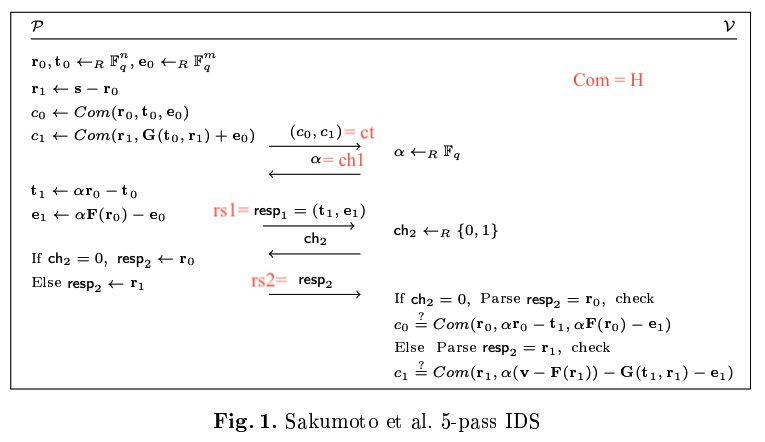
\includegraphics[width=1\textwidth]{5_pass_ids.png}
This finally implies knowledge error $k = \frac{1}{2}[1]+\frac{1}{2}[\frac{1}{q}] = \frac{1}{2} + \frac{1}{2q}$. This implies 5-pass has lesser knowledge error $k$ if $q\geq 4$.\\

$\textbf{Pros and Cons in signature construction from 5-pass IDS:}$ We will take 3-pass based MQ-DSS as benchmark to compare 5-pass IDS based MQ-DSS.\\
$\bullet$ Knowledge error $k$ criteria: 3-pass has fixed knowledge error of $\frac{2}{3}$. While 5-pass has $k = \frac{1}{2} + \frac{1}{2q}$. Hence, it can do better if $q\geq4$. Since on running $r$ rounds, knowledge error goes like $k^r$. Hence, small $k$ implies comparatively smaller $r$ required to achieve negligible error. Also the value of $r$ directly proportional to the size of signature generated. Hence, 5-pass has an advantage over 3-pass. It is important to note that we can't make $q$ arbitrary large as it will increase the transcript size per round too. The optimal $q$ is achieved for $\mathbb{F}_q = \mathbb{F}_{31}$. \footnote{https://eprint.iacr.org/2016/708.pdf ,Page-21} \\
$\bullet$ Extractor for computing witness: We have seen three accepted special transcript is sufficient for getting a witness for 3-pass IDS. But, 5-pass IDS requires five such transcripts to extract a witness. Hence, another layer of complexity is added for adversary $\mathcal{A}.$ 


\section*{Acknowledgement}
$\bullet$ Most of the idea is taken from the classroom lecture slides.\\
$\bullet$ Fig.1 is taken from the paper \hyperlink{https://eprint.iacr.org/2016/708.pdf}{Schwabe et.al(2016)}.\\
$\bullet$ A few ideas from \hyperlink{https://2017.pqcrypto.org/school/schedule.html}{Post-Quantum Cryptography 2017 Summer School on Post-Quantum Cryptography 2017}.
\\
$\bullet$ This document is pdf version of the $\mathbb{LATEX}$ code written on \hyperlink{https://www.overleaf.com/read/tmqfgrkddzkj}{Overleaf}.\\
\begin{center}
   $\mathcal{THANK\ YOU}$
\end{center} 
                                       



\end{document}